\section{Results}

For the given experimental setting, impressive results were obtained for all aforementioned ablations. Hyperparameter tuning of the baseline model for input channels $c_{1;in}$ and learning rate $\gamma$ achieved improved performance compared to leading contemporary research in 3-class Dice measures with top-$97.71$ and $+1.277$ gain \cite{BBBC039ResearchStudy}. See Table \ref{tab:main} for a detailed list of results across the 50 separate model variations.


\subsection{Loss Convergence}

Each model converged similarly for the Cross-Entropy loss as shown in Figure \ref{fig:loss-convergence}. There was no major variation between training and validation loss other than the immediate decrease indicating an efficient convergence to a localised minima. The RandAugment hyperparameter $n$ mainly impacted the magnitude of loss due to the introduced noise from augmentation operations such as the fill space in \textit{translate} and \textit{rotate} creating easily inferable null classes. Loss converged slowly indicating the ease of learning nuclei features, but was constrained by the third class boundaries reinforced by the large difference between 3-/2-channel AJI results from Table \ref{tab:main}. High variation in loss convergence is shared across all augmentation policies but there is clearly perturbations as $n$ increases alongside less efficient decline in loss.

\begin{figure}[h]
    \centering
    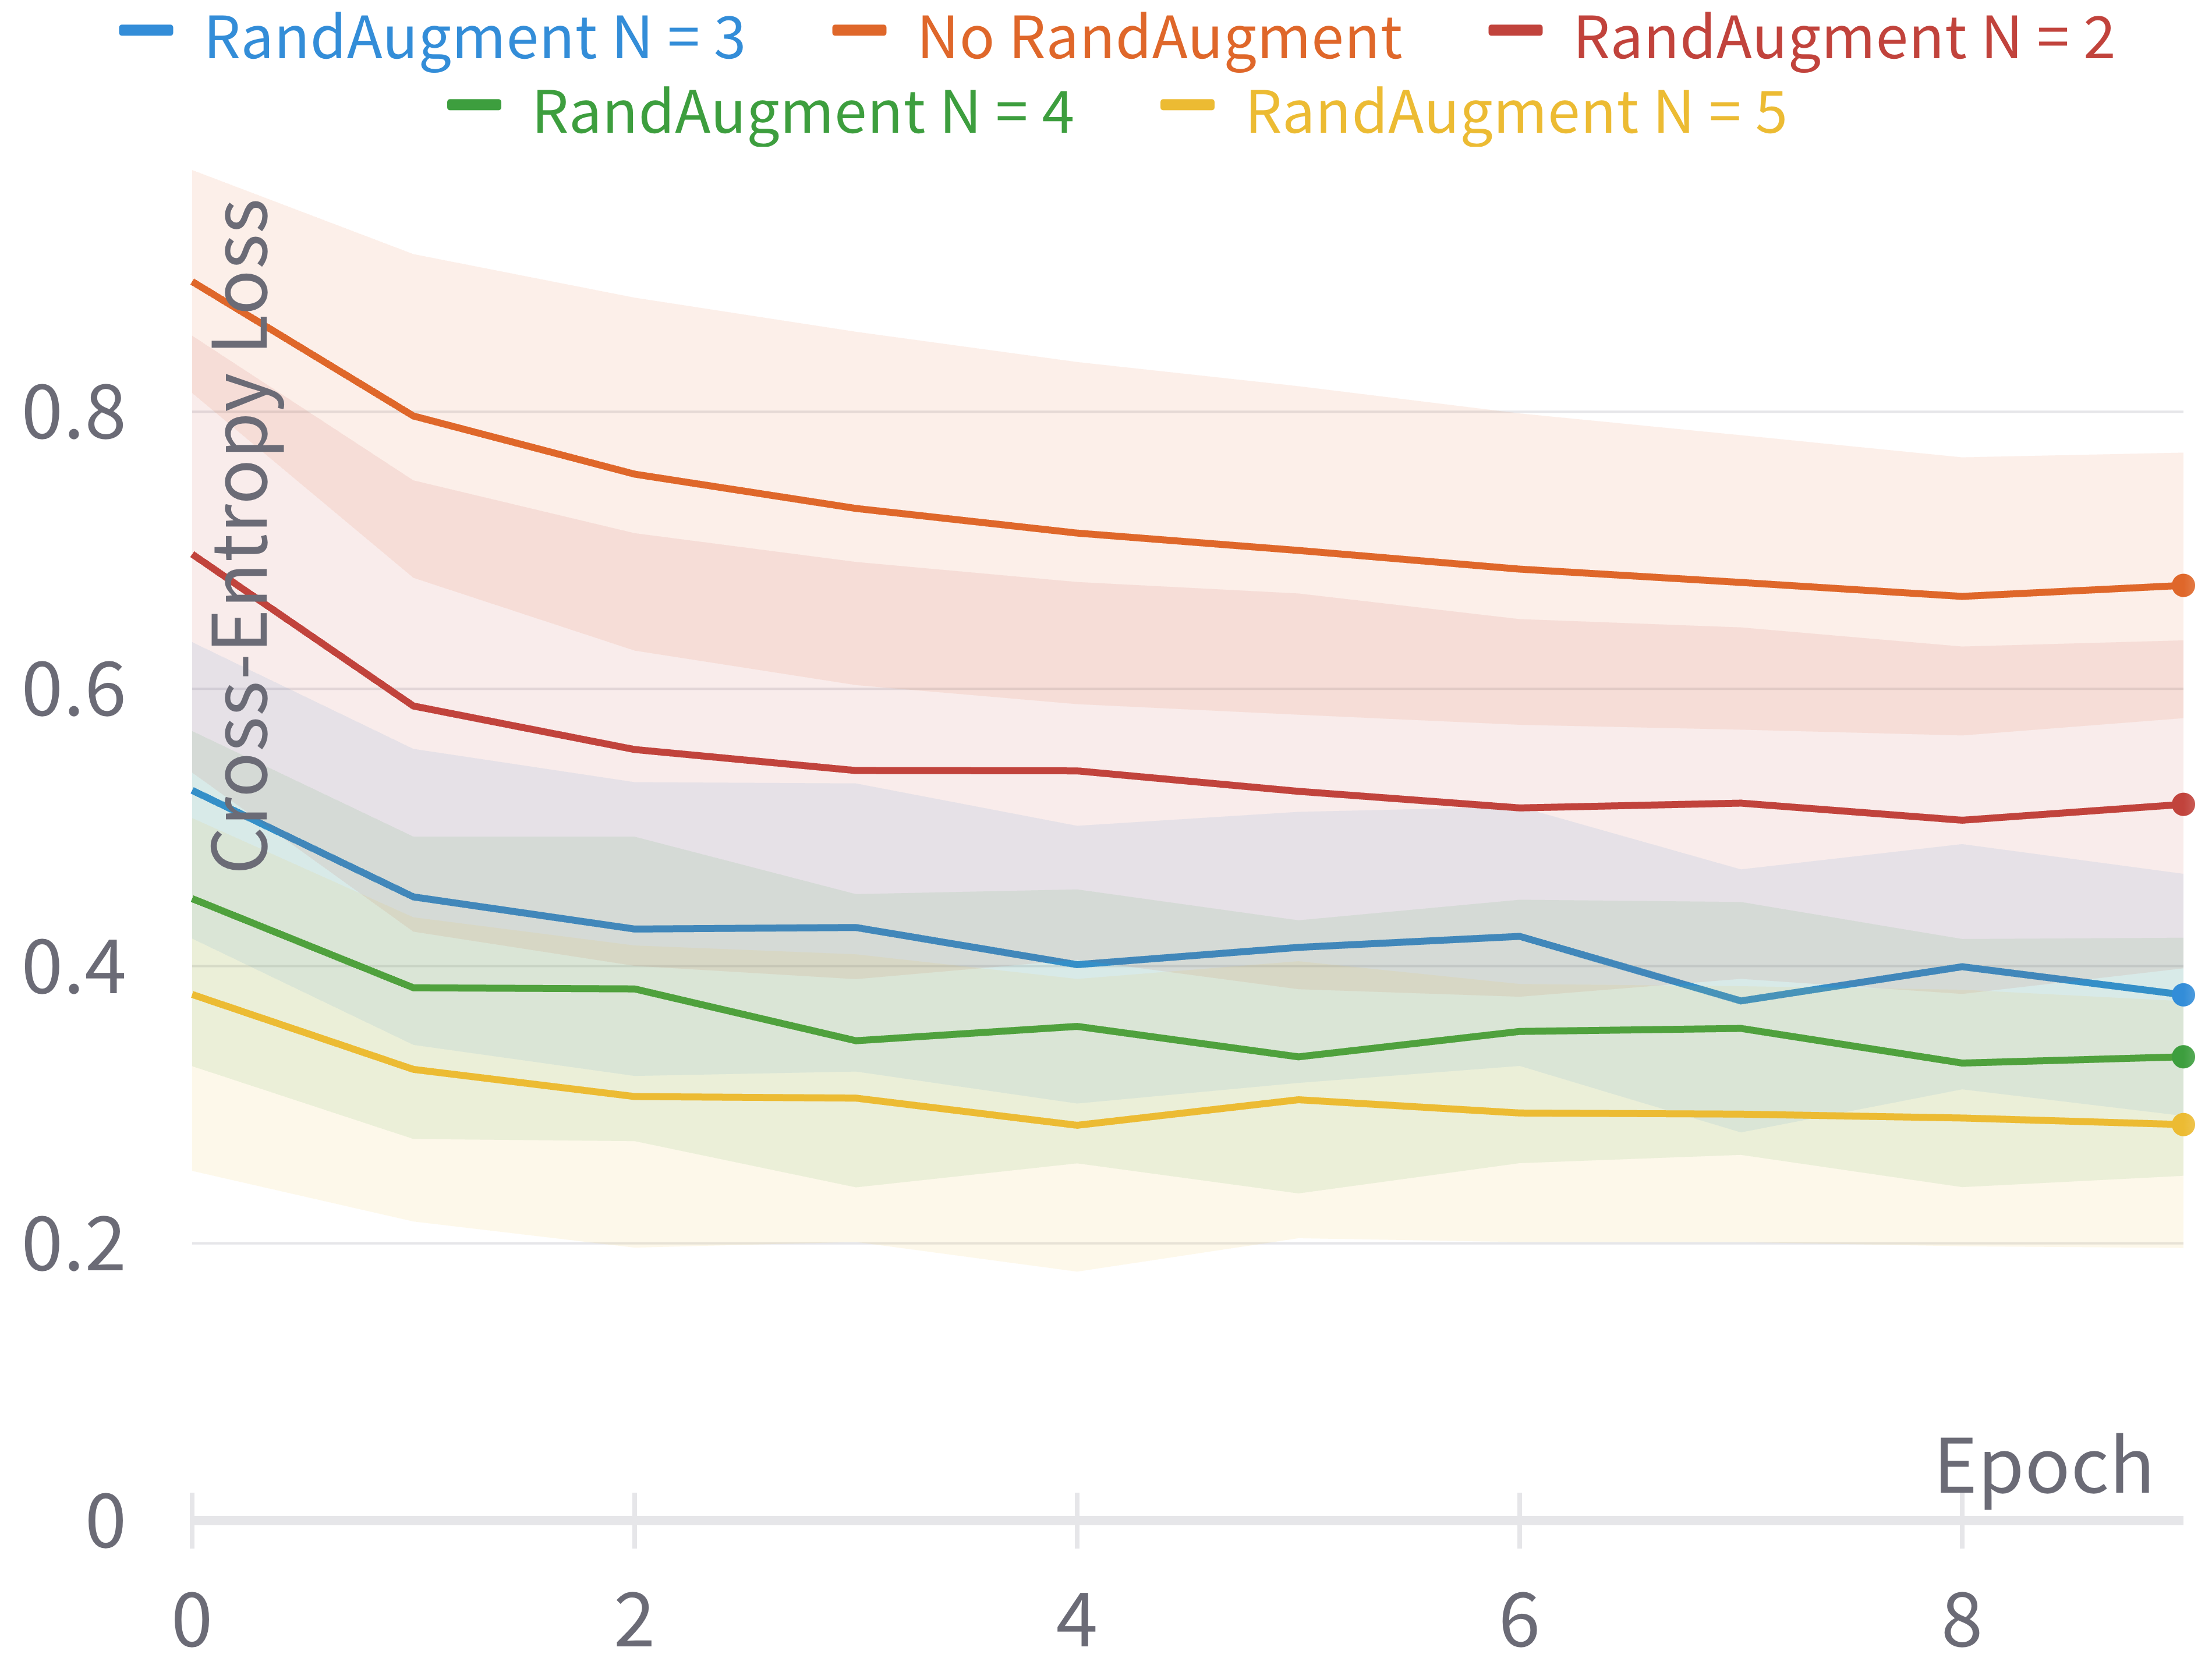
\includegraphics[width=0.7\linewidth]{figures/train_loss.png}
    \caption*{a) Training loss}
    \vspace{0.8em}
    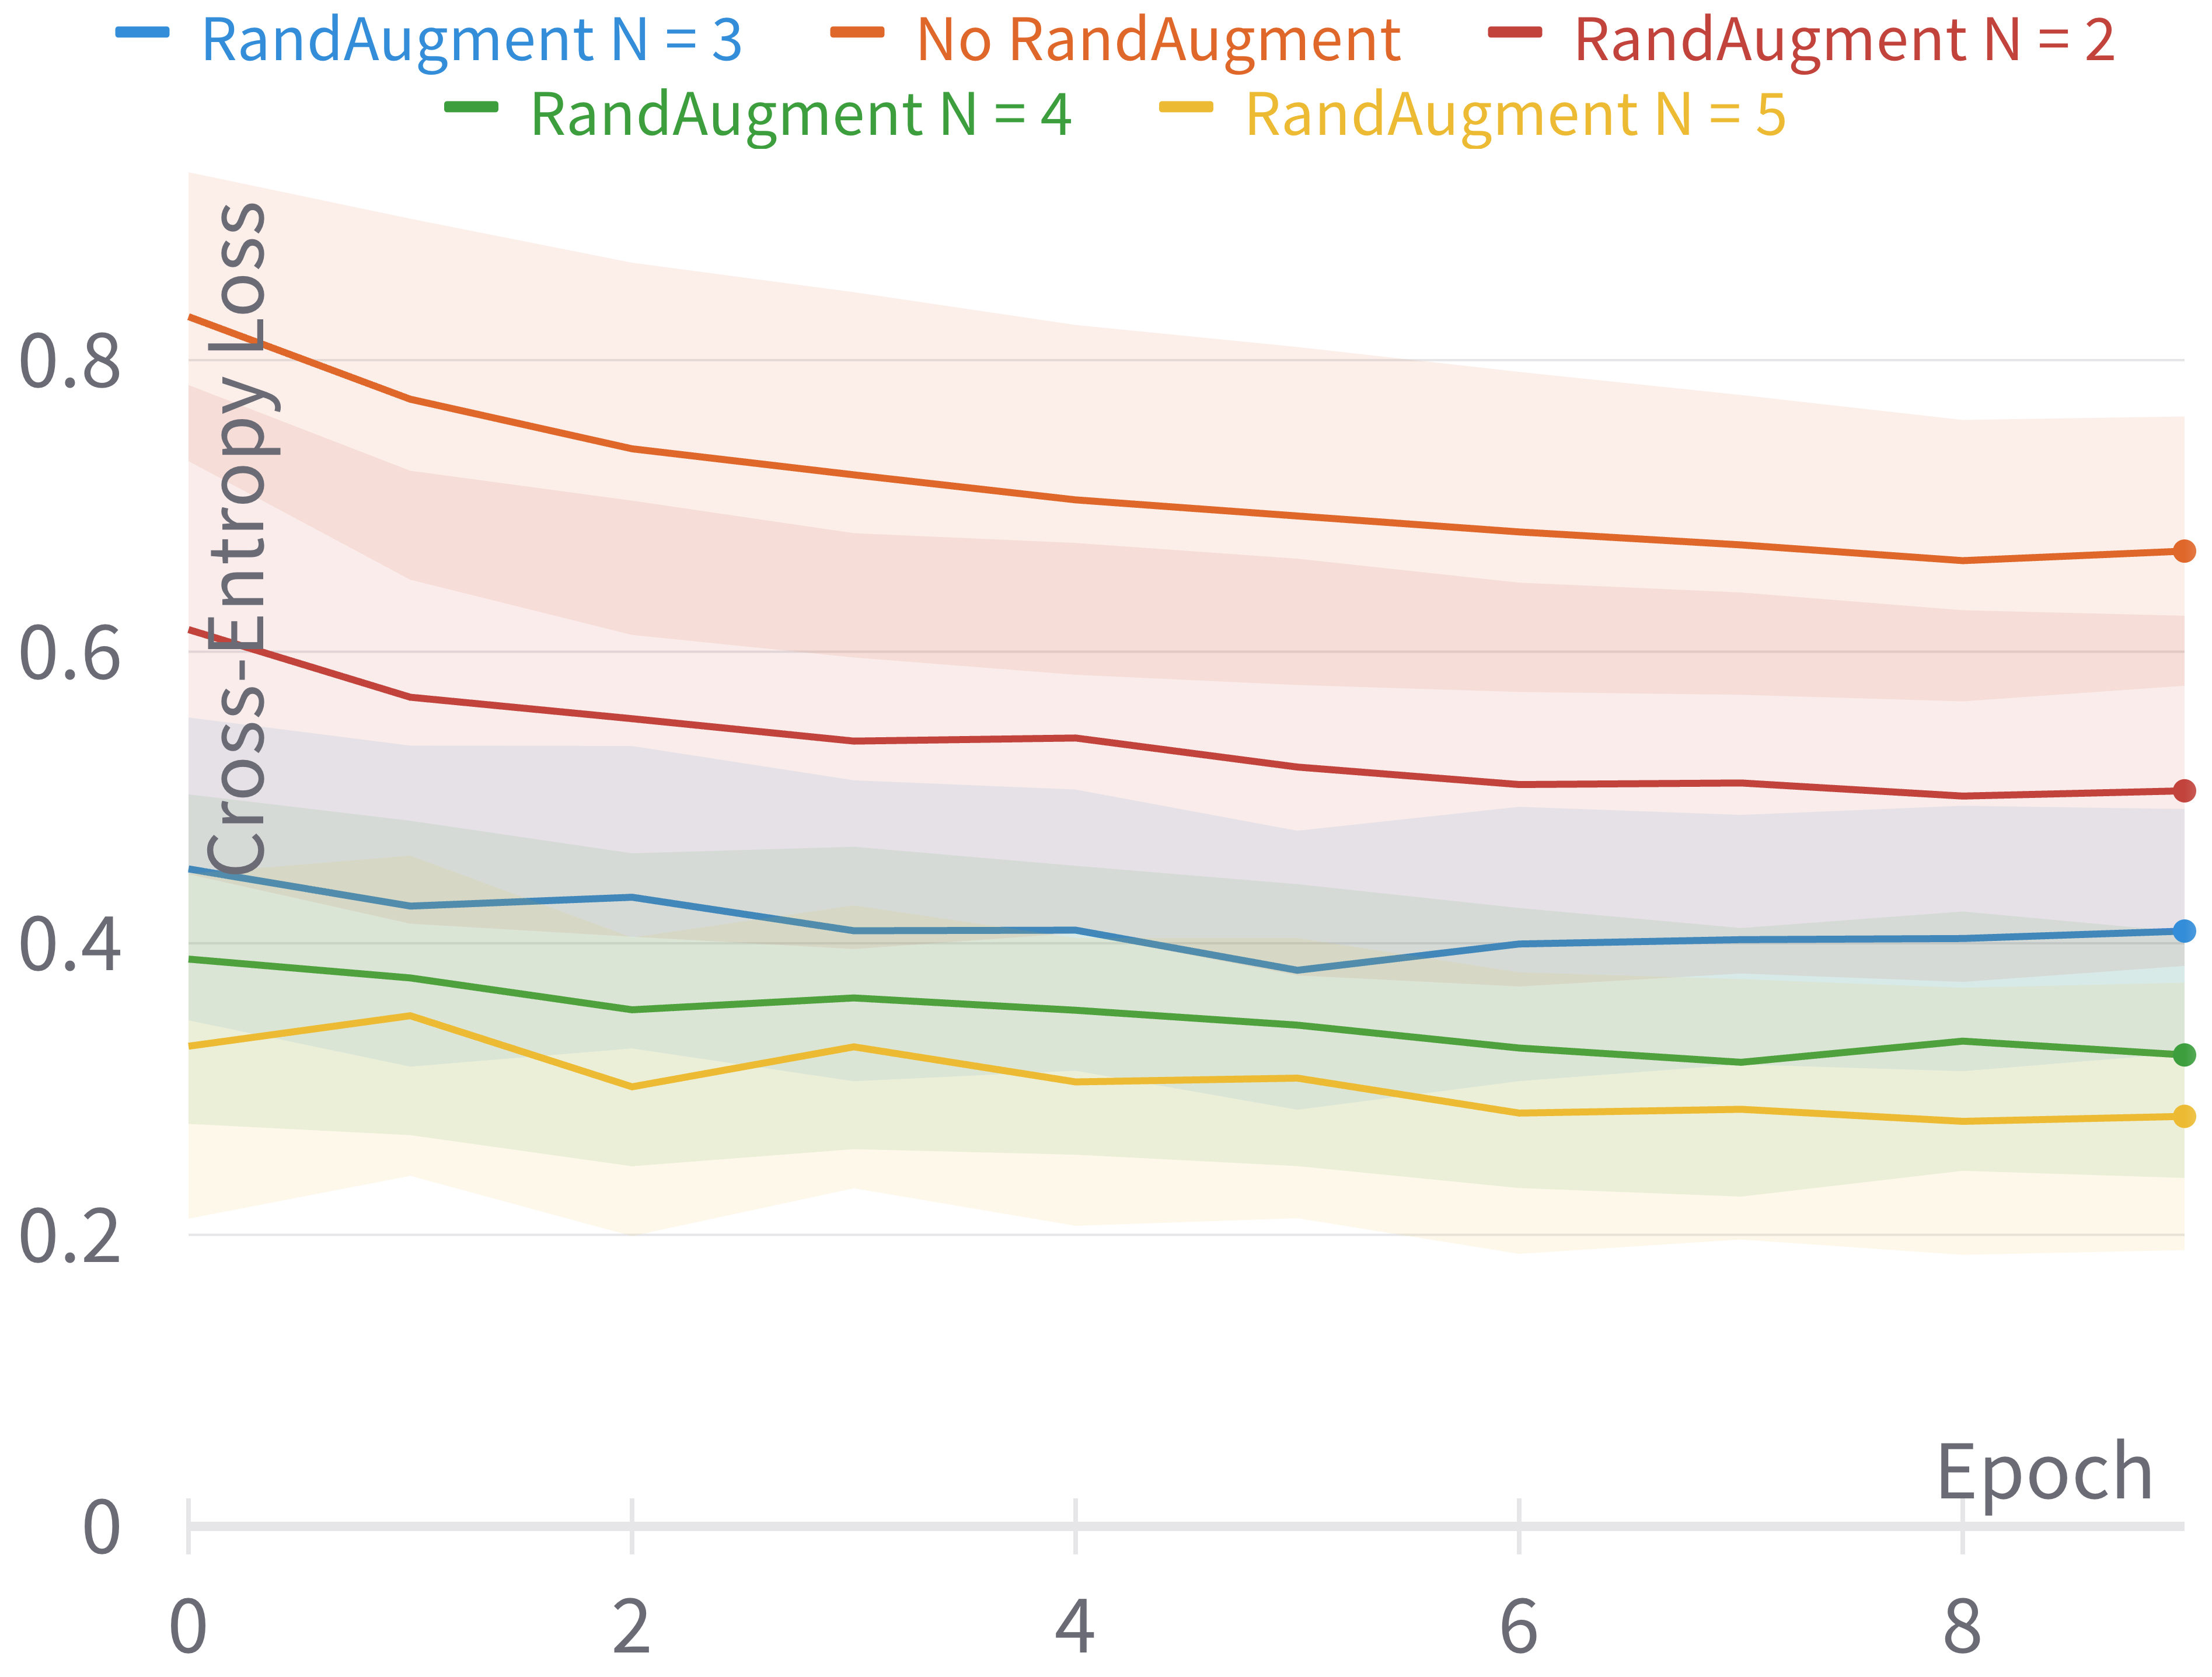
\includegraphics[width=0.7\linewidth]{figures/val_loss.png}
    \caption*{b) Validation loss}
    \caption{Cross-entropy loss convergence for U-Net DLA grouped by RandAugment $n$ per epoch for training and validation subsets.}
    \label{fig:loss-convergence}
\end{figure}

\begin{figure*}[h]
    \centering
    \includegraphics*[width=\textwidth]{figures/parameter_selection.png}
    \caption{U-Net DLA AJI parallel coordinates plot for hyperparameter ablation comparisons.}
    \label{fig:parameter-selection}
\end{figure*}

\subsection{Hyperparameter Selection}

Foundational hyperparameters for this experiment include the initial features $c_{1;in}$, learning rate $\gamma$, and modified RandAugment $n,m$ parameters. Figure \ref{fig:parameter-selection} shows the impact of different hyperparameters on the test Aggregate Jaccard Index (AJI). There is a clear correlation for $\gamma$ preferencing higher learning rates, although Table \ref{tab:main} shows that top-performing models vary consistently between both values highlighting correlative dependency with other parameters. Additionally, there is a greater impact from the number of operations $n$ over the scalar magnitude $m$ where reduced operations, although showing variable results, lead to greater performing models. There is increased variance introduced with expressive augmentation policies which is expected by impacting convolutional bottlenecks under different $c_{1;in}$ and $\gamma$ parameters. 

The optimal configuration for the RandAugment policy must balance the bias-variance trade-off and leverage a stable combination; $n=3$ and $m=0.25$ yields the optimal results. This is reinforced by Figure \ref{fig:randaug-f1} where final test top-$F_1$ scores were attained by this combination. Consequently, increase variation was observed for $n$ having skewed performance but the decrease deviation $\sigma$ for $m$ indicates greater stability over $m=0.5$ and improved performance over $m=0.1$, a similar result being observed for $n$. 

Finally, selection of $c_{1;in}$ was more difficult due to the inter-correlation between other hyperparameters. Increase network parameters allows greater propagation of noise from harsher augmentation policies and so smaller networks are preferenced, although mid-range policies can allow for larger models to have stable convergence. Therefore, a bigger network with $c_{1;in} = 64$ can be matched with the chosen RandAugment configuration. 

Conferring with Table \ref{tab:main} as a consistently high performing model across the listed evaluation metrics, the optimal hyperparameter configuration chosen for the U-Net DLA model uses $c_{1;in}=64$, $\gamma=0.0001$, $n=3$, and $m=0.25$. Following a final testing loop for $E=30$ epochs, the model attained $90.37/65.39\%$ accuracy, $97.71/98.77$ Dice, $84.37/97.96$ AJI, and $90.60/65.98$ $F_1$.


\begin{figure}
    \centering
    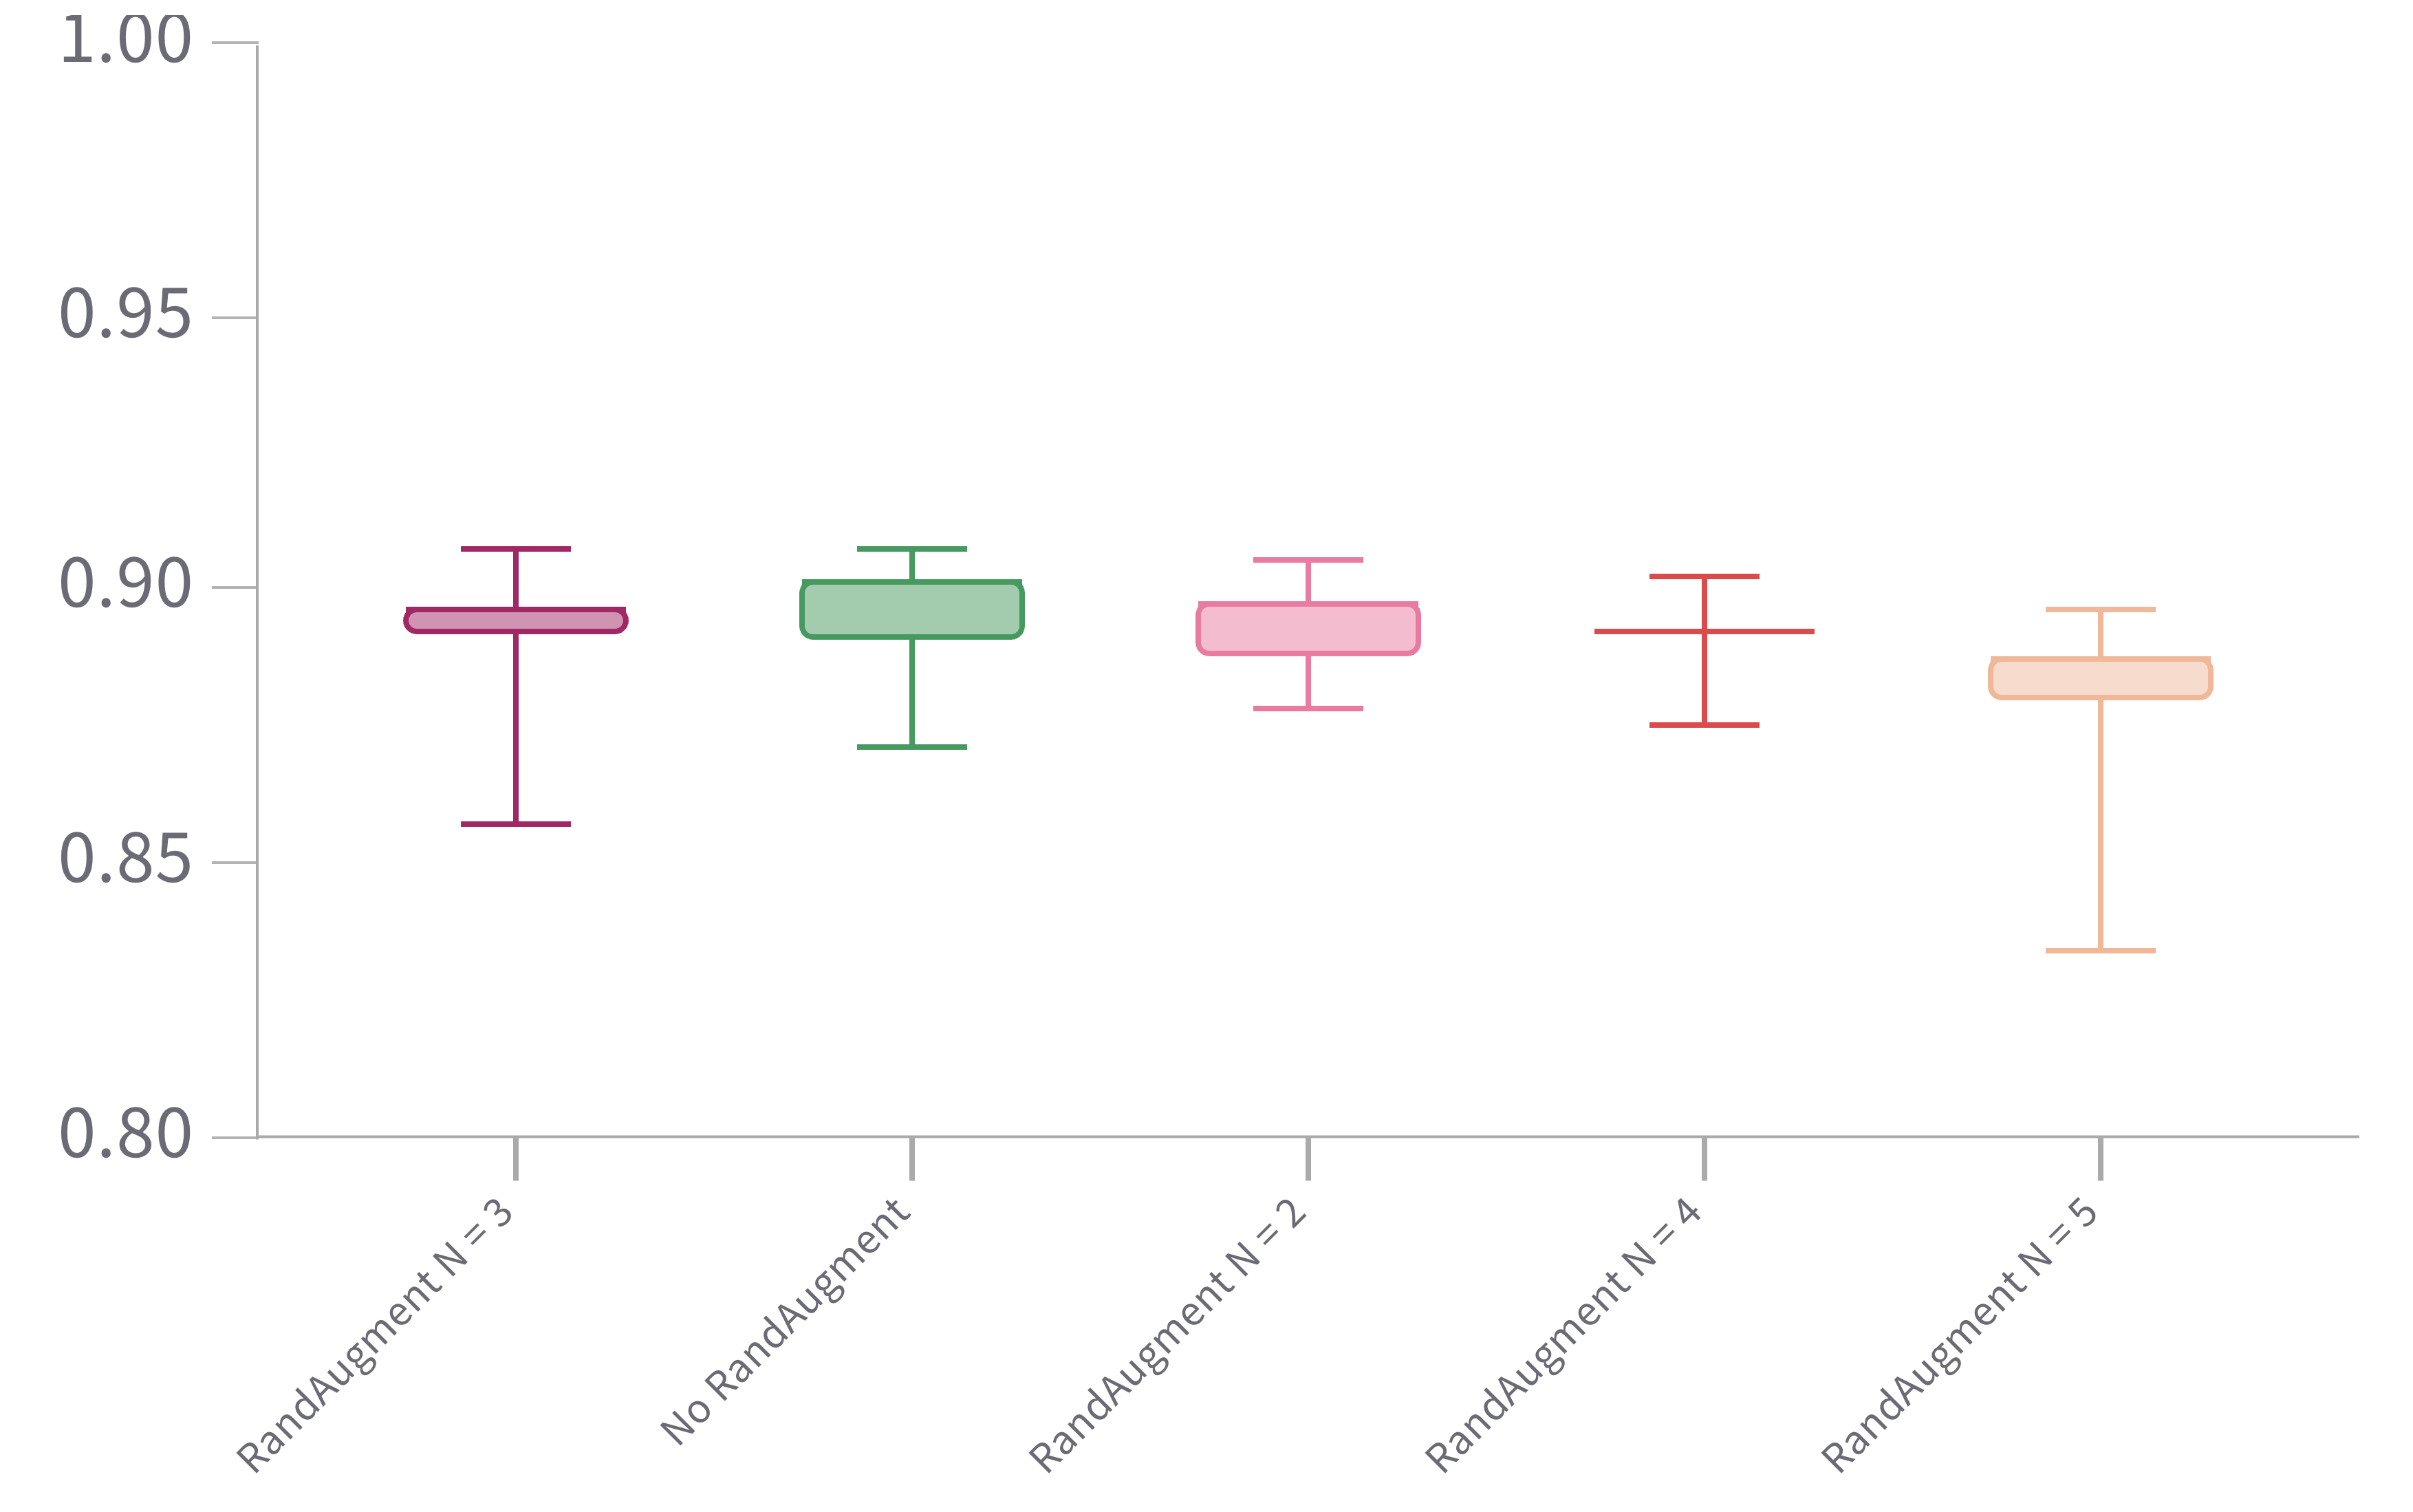
\includegraphics[width=0.9\linewidth]{figures/randaugment_n_f1.png}
    \caption*{a) RandAugment $n$}
    \vspace{1em}
    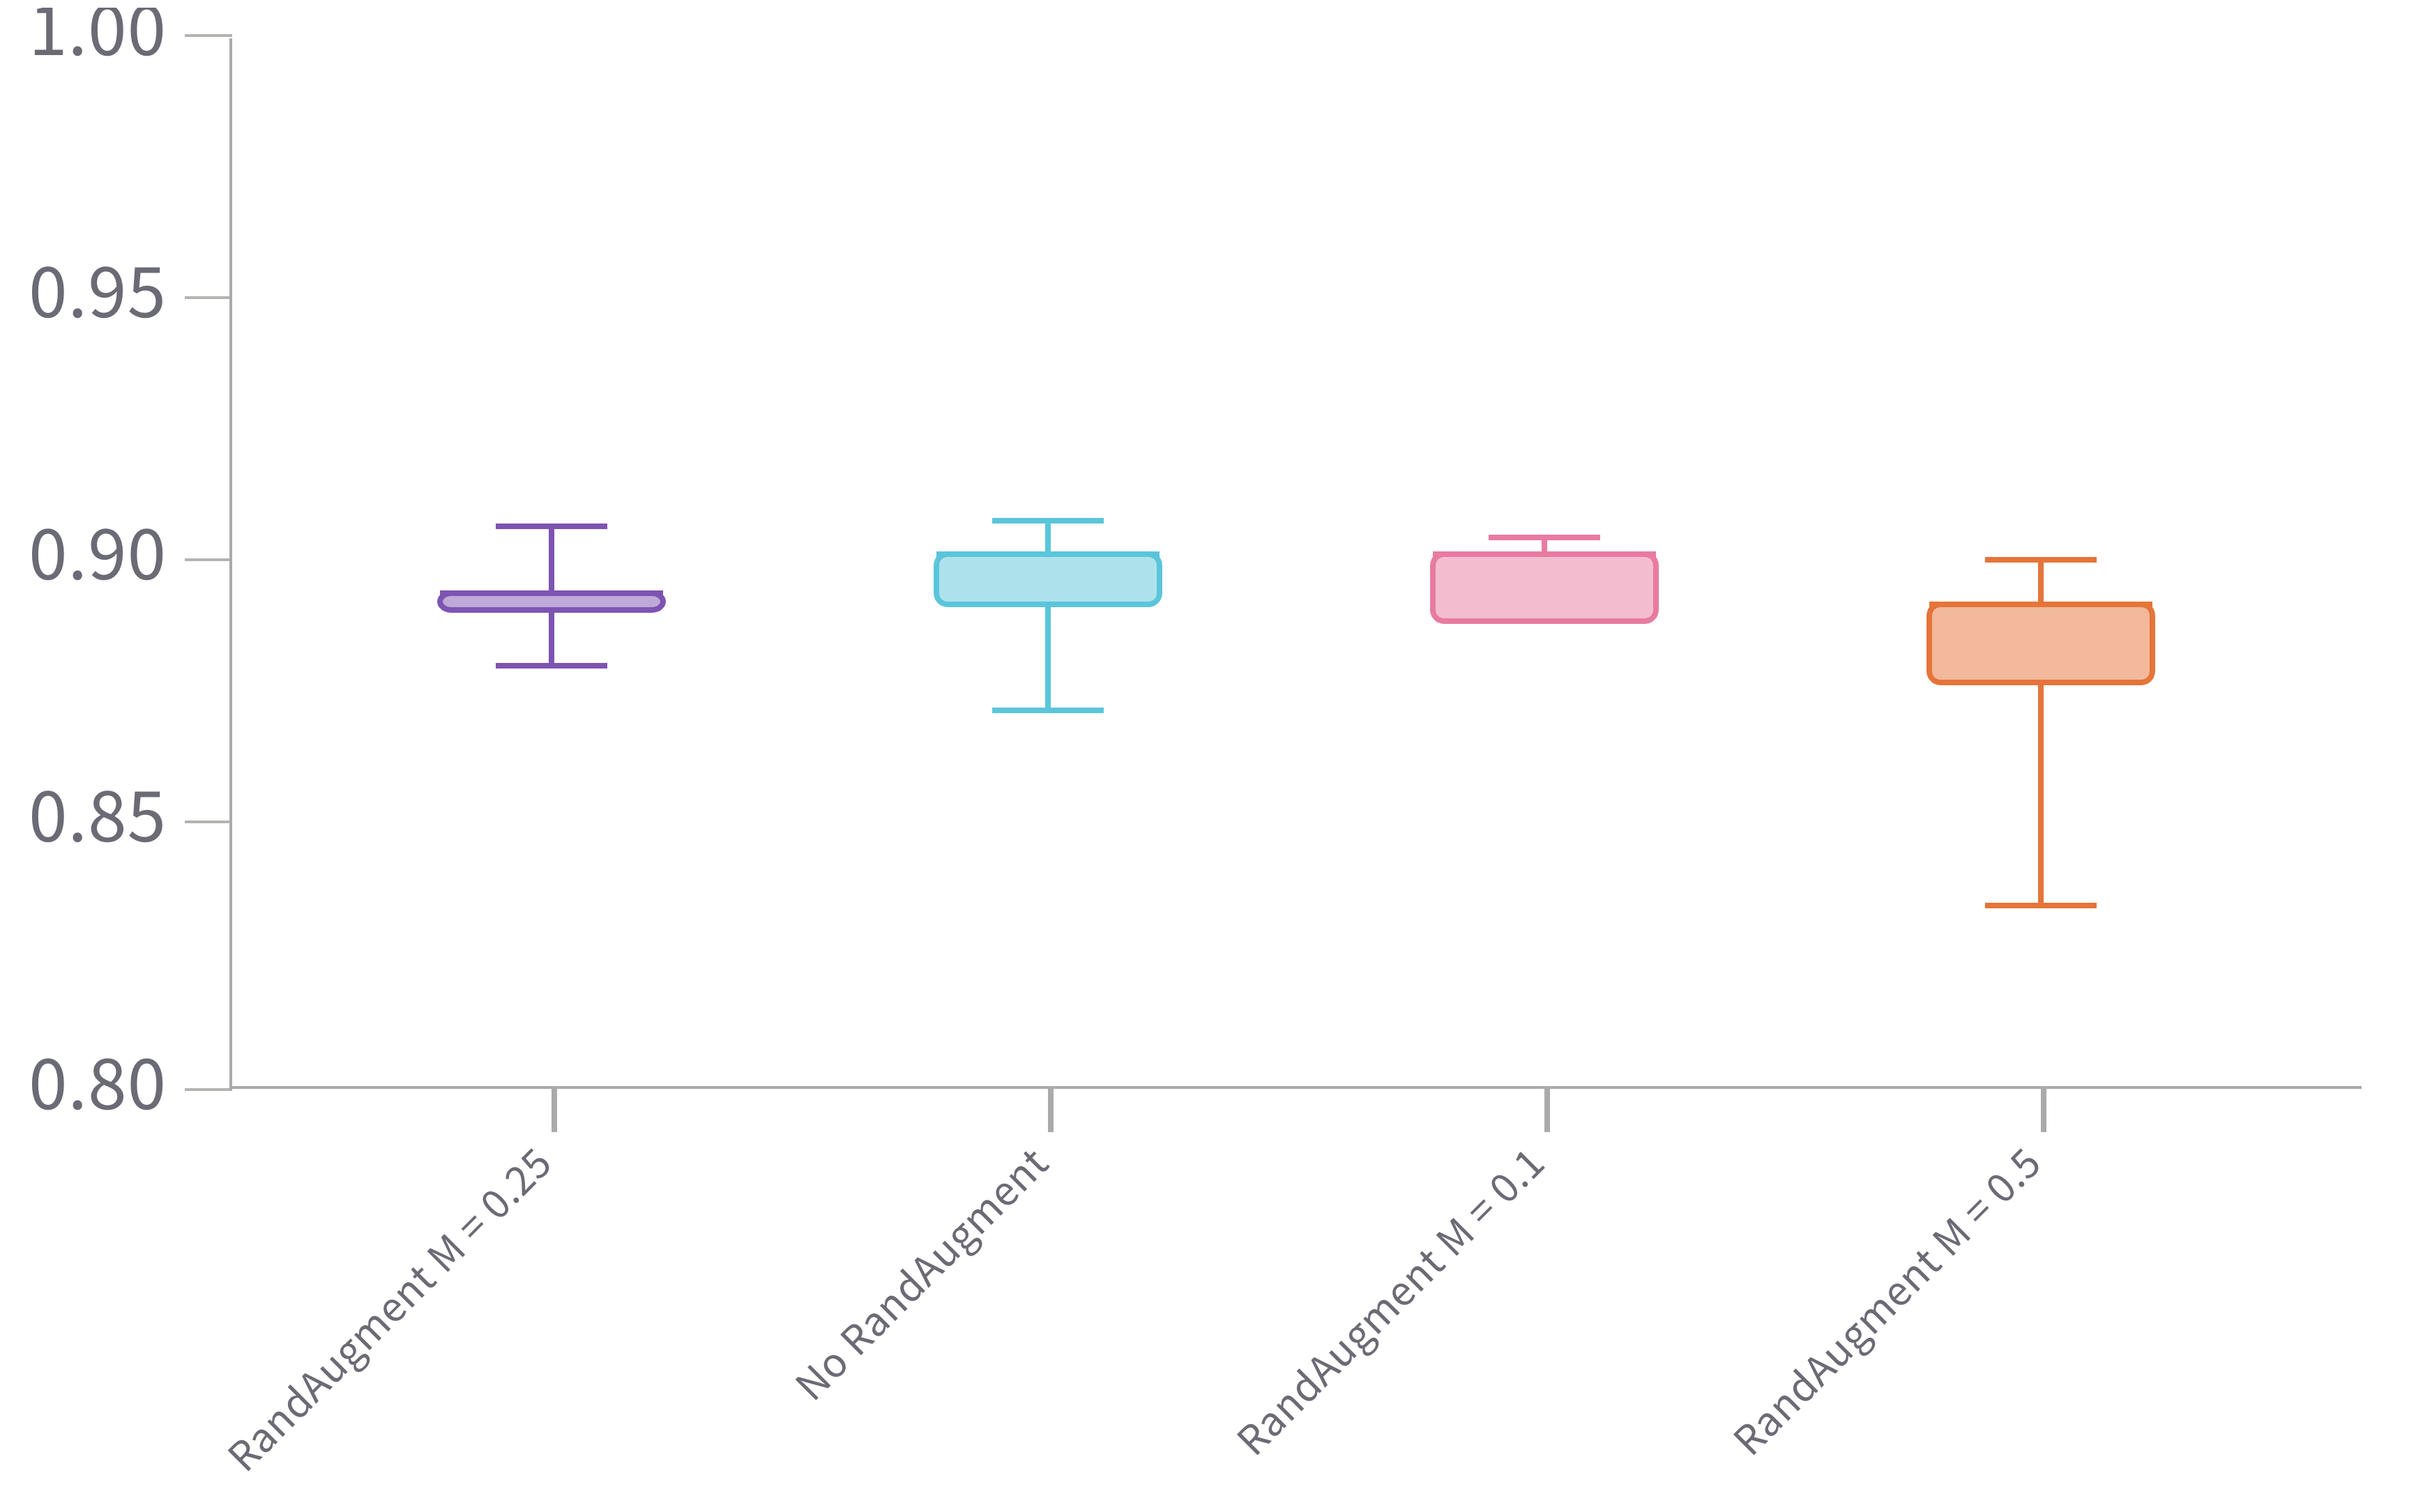
\includegraphics[width=0.9\linewidth]{figures/randaugment_m_f1.png}
    \caption*{b) RandAugment $m$}
    \caption{U-Net DLA final test $F_1$ performance across RandAugment hyperparameters $n,m$.}
    \label{fig:randaug-f1}
\end{figure}


\begin{table*}
    \caption{Summary of model evaluation metrics for all tuned hyperparameters; metrics marked in bold are top 3- or 2-channel results for the baseline/modified RandAugment group. Metrics show 3-/2-class results (with/without the boundary class).}
    \label{tab:main}
    \begin{tabular}{l|rr|rr|llll}
    \toprule
    & $N$-Ftrs & LR & RA-$n$ & RA-$m$ & Accuracy & Dice & $AJI$ & $F_1$ \\
    \midrule
                & 16 & 0.0001    & - & - & \textbf{92.45/64.66}  & 96.96/98.37   & 82.36/96.89    & 89.14/65.61 \\
                & 16 & 0.001     & - & - & 90.73/65.24  & \textbf{97.73/98.78}   & 84.60/97.76     & \textbf{90.78/65.91} \\
                & 32 & 0.0001    & - & - & 90.15/64.99  & 97.59/98.69   & 83.80/97.35     & 90.22/65.76 \\
                & 32 & 0.001     & - & - & 87.08/65.66  & 96.93/98.34   & \textbf{79.81/98.22}    & 87.12/66.07 \\
                & 64 & 0.0001    & - & - & 91.50/65.22  & 97.58/98.70   & 84.22/97.72    & 90.51/65.89 \\
    Baseline    & 64 & 0.001     & - & - & 88.96/65.31  & 97.67/98.74   & 83.83/97.86    & 90.19/65.94 \\
    \midrule
                & 16    & 0.0001    & 2  & 0.10     & 92.40/63.61   & 96.88/98.33    & 81.80/95.36   & 88.84/65.07   \\
                & 16    & 0.001     & 2  & 0.10     & 90.77/64.55   & 97.50/98.65    & 83.65/96.72   & 90.14/65.54   \\
                & 32    & 0.0001    & 2  & 0.10     & 90.05/65.35   & \textbf{97.68/98.75}    & 84.12/97.89   & 90.43/65.95   \\
                & 32    & 0.001     & 2  & 0.10      & 91.85/64.11   & 97.16/98.48    & 82.66/96.09   & 89.44/65.32 \\
                & 64    & 0.001     & 2  & 0.25     & \textbf{92.94/63.90}   & 97.01/98.39    & 82.52/95.78   & 89.35/65.22   \\
                & 64    & 0.0001    & 2  & 0.25     & 90.67/65.13   & 97.66/98.74    & 84.31/97.58   & \textbf{90.57/65.85}   \\
                & 64    & 0.001     & 2  & 0.50     & 90.54/64.25   & 97.39/98.60    & 83.11/96.29   & 89.76/65.39   \\
                Mod-RA & 64    & 0.0001    & 2  & 0.50     & 87.82/65.57   & 97.07/98.42    & \textbf{80.64/98.19}   & 87.79/66.06   \\
                \midrule
                & 16    & 0.0001    & 3  & 0.50     & 90.17/62.69   & 96.68/98.21    & 80.16/93.98   & 87.70/64.55    \\
                & 16    & 0.001     & 3  & 0.25     & 92.55/64.36   & 96.99/98.39    & 82.45/96.47   & 89.24/65.46   \\
                & 32    & 0.0001    & 3  & 0.25     & 91.52/64.80   & 97.41/98.61    & 83.53/97.10   & 90.03/65.68   \\
                & 32    & 0.001     & 3  & 0.25     & 88.84/65.64   & 97.50/98.65    & \textbf{82.78/98.32}   & 89.42/66.10    \\
                & 64    & 0.0001    & 3  & 0.25     & \textbf{91.73/64.95}   & \textbf{97.62/98.72}    & 84.46/97.32   & \textbf{90.70/65.76}    \\
                & 64    & 0.001     & 3  & 0.25     & 89.74/65.40   & 97.55/98.68    & 83.43/97.96   & 89.92/65.98   \\
                & 16    & 0.0001    & 3  & 0.50     & 91.08/64.72   & 97.14/98.46    & 82.46/96.97   & 89.22/65.64   \\
                & 16    & 0.001     & 3  & 0.50     & 89.65/65.34   & 97.54/98.67    & 83.40/97.89   & 89.89/65.95   \\
                & 32    & 0.0001    & 3  & 0.50     & 87.28/65.40   & 96.39/98.06    & 78.18/97.93   & 85.76/65.97   \\
                & 32    & 0.001     & 3  & 0.50     & 89.94/65.18   & 97.43/98.62    & 83.05/97.66   & 89.64/65.88   \\
                & 64    & 0.001     & 3  & 0.50     & 89.88/64.87   & 97.53/98.67    & 83.49/97.20   & 89.99/65.71   \\
                Mod-RA & 64    & 0.0001    & 3  & 0.50     & 88.64/65.34   & 97.51/98.65    & 82.95/97.87   & 89.54/65.95   \\
                \midrule
                & 16    & 0.001     & 4  & 0.25     & \textbf{92.22/63.73}   & 96.70/98.23    & 81.28/95.54   & 88.42/65.13   \\
                & 16    & 0.0001    & 4  & 0.25     & 89.58/64.42   & 97.30/98.54    & 82.45/96.53   & 89.25/65.48   \\
                & 32    & 0.001     & 4  & 0.25     & 90.40/65.27   & 97.25/98.52    & 82.46/97.79   & 89.20/65.92    \\
                & 32    & 0.0001    & 4  & 0.25     & 89.33/65.43   & 97.51/98.66    & \textbf{83.04/98.03}   & 89.63/66.00    \\
                & 64    & 0.001     & 4  & 0.25     & 90.79/65.29   & \textbf{97.56/}98.69    & 83.84/97.83   & \textbf{90.22/65.93}   \\
                & 64    & 0.0001    & 4  & 0.25     & 89.70/65.42   & 97.49/98.65    & 83.18/97.99   & 89.73/65.99   \\
                & 16    & 0.001     & 4  & 0.50     & 89.16/63.30   & 96.62/98.13    & 80.06/94.82   & 87.53/64.87   \\
                & 16    & 0.0001    & 4  & 0.50     & 89.44/64.49   & 97.29/98.53    & 82.39/96.63   & 89.19/65.51   \\
                & 32    & 0.001     & 4  & 0.50     & 89.63/65.29   & 97.32/98.56    & 82.46/97.79   & 89.20/65.92    \\
                & 32    & 0.0001    & 4  & 0.50     & 90.42/65.02   & 97.30/98.54    & 82.70/97.42   & 89.41/65.79   \\
                & 64    & 0.001     & 4  & 0.50     & 90.64/64.67   & 97.41/98.61    & 83.22/96.91   & 89.81/65.61   \\
                Mod-RA & 64    & 0.0001    & 4  & 0.50     & 88.92/64.28   & 97.25/98.50    & 82.09/96.32   & 88.99/65.40   \\
                \midrule
                & 16    & 0.001     & 5  & 0.25     & \textbf{92.04/63.75}   & 96.55/98.15    & 80.80/95.56   & 88.04/65.14   \\
                & 16    & 0.0001    & 5  & 0.25     & 88.57/65.55   & 97.32/98.56    & 81.91/98.18   & 88.77/66.05   \\
                & 32    & 0.001     & 5  & 0.25     & 90.50/65.23   & \textbf{97.38/98.59}    & 83.03/97.72   & \textbf{89.63/65.90}   \\
                & 32    & 0.0001    & 5  & 0.25     & 89.43/65.45   & 97.37/98.58    & 82.51/98.04   & 89.24/66.01   \\
                & 64    & 0.001     & 5  & 0.25     & 91.13/64.87   & 97.09/98.44    & 82.23/97.21   & 89.05/65.72   \\
                & 64    & 0.0001    & 5  & 0.25     & 87.70/64.62   & 97.28/98.53    & 81.84/96.81   & 88.73/65.57   \\
                & 16    & 0.001     & 5  & 0.50     & 85.93/59.80   & 94.98/96.97    & 74.26/89.27   & 83.41/62.73   \\
                & 16    & 0.0001    & 5  & 0.50     & 87.79/64.85   & 97.27/98.53    & 81.65/97.18   & 88.59/65.70   \\
                & 32    & 0.001     & 5  & 0.50     & 89.61/62.56   & 96.51/98.12    & 79.45/93.77   & 87.15/64.47   \\
                & 32    & 0.0001    & 5  & 0.50     & 85.11/65.82   & 97.12/98.44    & \textbf{79.57/98.55}   & 86.86/66.18   \\
                & 64    & 0.001     & 5  & 0.50     & 88.25/64.93   & 97.12/98.45    & 81.17/97.26   & 88.23/65.73   \\
    Mod-RA & 64    & 0.0001    & 5  & 0.50     & 89.41/64.37   & 97.28/98.53    & 82.32/96.47   & 89.15/65.46   \\
    \bottomrule
    \end{tabular}
\end{table*}
